% begin module continuity-ex3
\begin{frame}
\begin{example} %[Example 3, p. 115]
Consider $f(x) = \lfloor x\rfloor$, and pick any integer $n$.
\begin{columns}[c]
\column{.4\textwidth}
\psset{xunit=1cm, yunit=1cm}
\begin{pspicture}(-1.5, -1.5)(3.8, 3.8)
\psframe*[linecolor=white](-1.5,-1.5)(3.8,3.8)
\psaxes[labels=x, ticks=x]{<->}(0,0)(-1.5,-1.5)(3.8,3.8)
\psline(-0.1,1)(0.1,1)
\rput[b](-0.25, 1){$1$}
\psline[linecolor=red](-1,-1)(0,-1)
\psFullDot{-1}{-1}
\psHollowDot{0}{-1}

\psline[linecolor=red](0,0)(1,0)
\psFullDot{0}{0}
\psHollowDot{1}{0}

\psline[linecolor=red](1,1)(2,1)
\psFullDot{1}{1}
\psHollowDot{2}{1}

\psline[linecolor=red](2,2)(3,2)
\psFullDot{2}{2}
\psHollowDot{3}{2}

\psline[linecolor=red](3,3)(3.8,3)
\psFullDot{3}{3}
%\psHollowDot{4}{3}
\end{pspicture} %
%\ 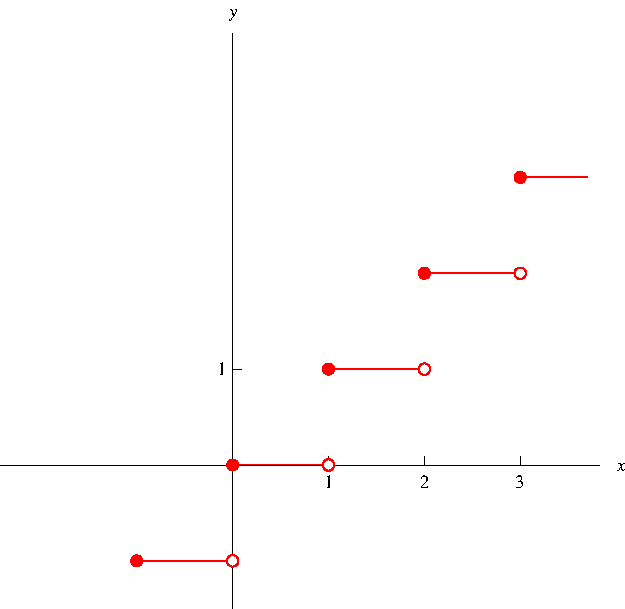
\includegraphics[height=4.5cm]{continuity/pictures/02-05-ex2d.pdf}%
\column{.6\textwidth}
\begin{itemize}
\item<2-| alert@3-4>  $f(n) = $ \uncover<4->{$n$.}
\item<2-| alert@5-6>  $\lim\limits_{x\rightarrow n^+} f(x) = $ \uncover<6->{$n$.}
\item<7->  Continuous from the right at $n$.
\item<2-| alert@8-9>  $\lim\limits_{x\rightarrow n^-} f(x) = $ \uncover<9->{$n-1$.}
\item<10->  Discontinuous from the left at $n$.
\end{itemize}
\end{columns}
\end{example}
\end{frame}
% end module continuity-ex3
